\documentclass[journal,11pt,onecolumn]{IEEEtran}

% Page configurations

\title{GATE 2016 - MECHANICAL ENGINEERING}

\usepackage[a4paper,bottom=1in,top=1in]{geometry}

\usepackage{amsmath}

\usepackage{graphicx}

\usepackage{float}

\usepackage{tikz}

\usepackage{multicol}

\setlength{\columnsep}{1cm}

% \usepackage{gvv-book}

\usepackage{gvv}

\usetikzlibrary{arrows}

\usetikzlibrary{decorations.markings}

\graphicspath{{figs/}}

\begin{document}

\begin{center}

    \Large

    \textbf{GATE 2016}

    \vspace{0.5cm}

    \textbf{MECHANICAL ENGINEERING (ME)}

\end{center}

\textit{Duration} : Three hours

\hfill

\textit{Maximum Marks} : 100

\large\textbf{General Aptitude - GA (Q.1 to Q.10)}\\

\normalsize\textbf{Q. 1 – Q. 5 carry one mark each.}\\

\begin{enumerate}

    \item Which of the following is CORRECT with respect to grammar and usage?

          Mount Everest is \_\_\_\_\_\_\_\_\_\_\_\_.

          \begin{enumerate}

              \begin{multicols}{2}

                  \item the highest peak in the world

                  \item highest peak in the world

                  \item one of highest peak in the world

                  \item one of the highest peak in the world

              \end{multicols}

          \end{enumerate}

    \item The policeman asked the victim of a theft, "What did you \_\_\_\_\_\_\_\_\_\_\_?"

          \begin{enumerate}

              \begin{multicols}{4}

                  \item loose

                  \item lose

                  \item loss

                  \item louse

              \end{multicols}

          \end{enumerate}

    \item Despite the new medicine's \_\_\_\_\_\_\_\_\_\_\_\_ in treating diabetes, it is not \_\_\_\_\_\_\_\_\_\_\_\_widely.

          \begin{enumerate}

              \item effectiveness --- prescribed

              \item availability --- used

              \item prescription --- available

              \item acceptance --- proscribed

          \end{enumerate}

    \item In a huge pile of apples and oranges, both ripe and unripe mixed together, 15\% are unripe fruits. Of the unripe fruits, 45\% are apples. Of the ripe ones, 66\% are oranges. If the pile contains a total of 5692000 fruits, how many of them are apples?

          \begin{enumerate}

              \begin{multicols}{2}

                  \item 2029198

                  \item 2467482

                  \item 2789080

                  \item 3577422

              \end{multicols}

          \end{enumerate}

    \item Michael lives 10 km away from where I live. Ahmed lives 5 km away and Susan lives 7 km away from where I live. Arun is farther away than Ahmed but closer than Susan from where I live. From the information provided here, what is one possible distance (in km) at which I live from Arun's place?

          \begin{enumerate}

              \begin{multicols}{4}

                  \item 3.00

                  \item 4.99

                  \item 6.02

                  \item 7.01

              \end{multicols}

          \end{enumerate}

\end{enumerate}

\normalsize\textbf{Q. 6 – Q. 10 carry two marks each.}\\

\begin{enumerate}[resume]

    \item A person moving through a tuberculosis prone zone has a 50\% probability of becoming infected. However, only 30\% of infected people develop the disease. What percentage of people moving through a tuberculosis prone zone remains infected but does not show symptoms of disease?

          \begin{enumerate}

              \begin{multicols}{4}

                  \item 15

                  \item 33

                  \item 35

                  \item 37

              \end{multicols}

          \end{enumerate}

    \item In a world filled with uncertainty, he was glad to have many good friends. He had always assisted them in times of need and was confident that they would reciprocate. However, the events of the last week proved him wrong.

          Which of the following inference(s) is/are logically valid and can be inferred from the above passage?

          (i) His friends were always asking him to help them.

          (ii) He felt that when in need of help, his friends would let him down.

          (iii) He was sure that his friends would help him when in need.

          (iv) His friends did not help him last week.

          \begin{enumerate}

              \item (i) and (ii)

              \item (iii) and (iv)

              \item (iii) only

              \item (iv) only

          \end{enumerate}

    \item Leela is older than her cousin Pavithra. Pavithra's brother Shiva is older than Leela. When Pavithra and Shiva are visiting Leela, all three like to play chess. Pavithra wins more often than Leela does.

          Which one of the following statements must be TRUE based on the above?

          \begin{enumerate}

              \item When Shiva plays chess with Leela and Pavithra, he often loses.

              \item Leela is the oldest of the three.

              \item Shiva is a better chess player than Pavithra.

              \item Pavithra is the youngest of the three.

          \end{enumerate}

    \item If $q^{-a}=\frac{1}{r}$ and $r^{-b}=\frac{1}{s}$ and $s^{-c}=\frac{1}{q}$, the value of $abc$ is \_\_\_\_\_\_\_\_.

          \begin{enumerate}

              \begin{multicols}{4}

                  \item $(rsq)^{-1}$

                  \item $0$

                  \item $1$

                  \item $r+q+s$

              \end{multicols}

          \end{enumerate}

    \item P, Q, R and S are working on a project. Q can finish the task in 25 days, working alone for 12 hours a day. R can finish the task in 50 days, working alone for 12 hours per day. Q worked 12 hours a day but took sick leave in the beginning for two days. R worked 18 hours a day on all days. What is the ratio of work done by Q and R after 7 days from the start of the project?

          \begin{enumerate}

              \begin{multicols}{4}

                  \item 10:11

                  \item 11:10

                  \item 20:21

                  \item 21:20

              \end{multicols}

          \end{enumerate}

\end{enumerate}
\begin{center}
    \Large
    \textbf{END OF THE QUESTION PAPER}
\end{center}

\pagebreak
\large\textbf{Mechanical Engineering - ME (Q.1 to Q.55)}\\

\normalsize\textbf{Q. 1 – Q. 25 carry one mark each.}\\

\begin{enumerate}

    \item The solution to the system of equations

          \[
              \myvec{2 & 5\\-4 & 3}\myvec{x\\y}=\myvec{2\\-30}
          \]

          is

          \begin{enumerate}
              \begin{multicols}{4}
                  \item $6, 2$
                  \item $-6, 2$
                  \item $-6, -2$
                  \item $6, -2$
              \end{multicols}

          \end{enumerate}

    \item If $f(t)$ is a function defined for all $t \geq 0$, its Laplace transform $F(s)$ is defined as

          \begin{enumerate}

              \begin{multicols}{2}

                  \item $\int_{0}^{\infty} e^{st} f(t) dt$

                  \item $\int_{0}^{\infty} e^{-st} f(t) dt$

                  \item $\int_{0}^{\infty} e^{ist} f(t) dt$

                  \item $\int_{0}^{\infty} e^{-ist} f(t) dt$

              \end{multicols}

          \end{enumerate}

    \item $f(z) = u(x,y) + iv(x,y)$ is an analytic function of complex variable $z = x + iy$ where $i = \sqrt{-1}$. If $u(x,y) = 2xy$, then $v(x,y)$ may be expressed as

          \begin{enumerate}

              \begin{multicols}{2}

                  \item $x^2 - y^2 + \text{constant}$

                  \item $y^2 - x^2 + \text{constant}$

                  \item $x^2 + y^2 + \text{constant}$

                  \item $-(x^2 + y^2) + \text{constant}$

              \end{multicols}

          \end{enumerate}

    \item Consider a Poisson distribution for the tossing of a biased coin. The mean for this distribution is $\mu$. The standard deviation for this distribution is given by

          \begin{enumerate}

              \begin{multicols}{4}

                  \item $\sqrt{\mu}$

                  \item $\mu^2$

                  \item $\mu$

                  \item $1/\mu$

              \end{multicols}

          \end{enumerate}

    \item Solve the equation $x^3 - x - 1 = 0$ using the Newton-Raphson method. The initial guess is $x_0 = 1$. The value of the predicted root after the first iteration, up to second decimal, is \_\_\_\_\_\_\_\_

    \item A rigid ball of weight 100 N is suspended with the help of a string. The ball is pulled by a horizontal force F such that the string makes an angle of 30° with the vertical. The magnitude of force F (in N) is \_\_\_\_\_\_\_\_

          \begin{figure}[H]
              \centering
              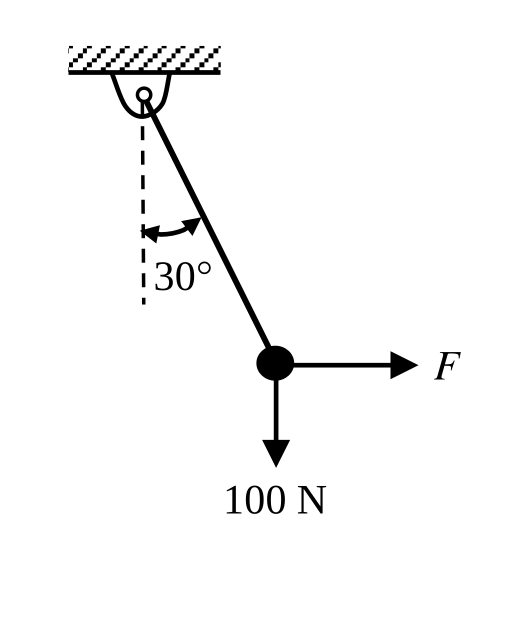
\includegraphics[scale=0.3]{q6}
              \caption{Figure for Q.6}
              \label{q6}
          \end{figure}

    \item A point mass M is released from rest and slides down a spherical bowl (of radius R) from a height H as shown in the figure below. The surface of the bowl is smooth (no friction). The velocity of the mass at the bottom of the bowl is

          \begin{figure}[H]
              \centering
              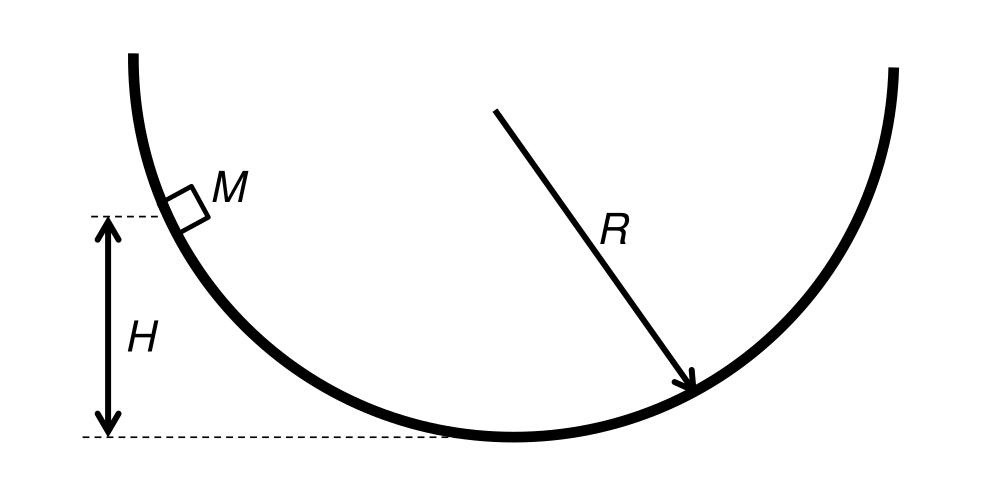
\includegraphics[scale=0.3]{q7}
              \caption{Figure for Q.7}
              \label{q7}
          \end{figure}

          \begin{enumerate}

              \begin{multicols}{4}

                  \item $\sqrt{gH}$

                  \item $\sqrt{2gH}$

                  \item $\sqrt{2gR}$

                  \item $0$

              \end{multicols}

          \end{enumerate}

    \item The cross sections of two hollow bars made of the same material are concentric circles as shown in the figure. It is given that $r_2 > r_1$ and $R_2 > R_1$, and that the areas of the cross-sections are the same. $J_1$ and $J_2$ are the torsional rigidities of the bars on the left and right, respectively. The ratio $J_2/J_1$ is

          \begin{figure}[H]
              \centering
              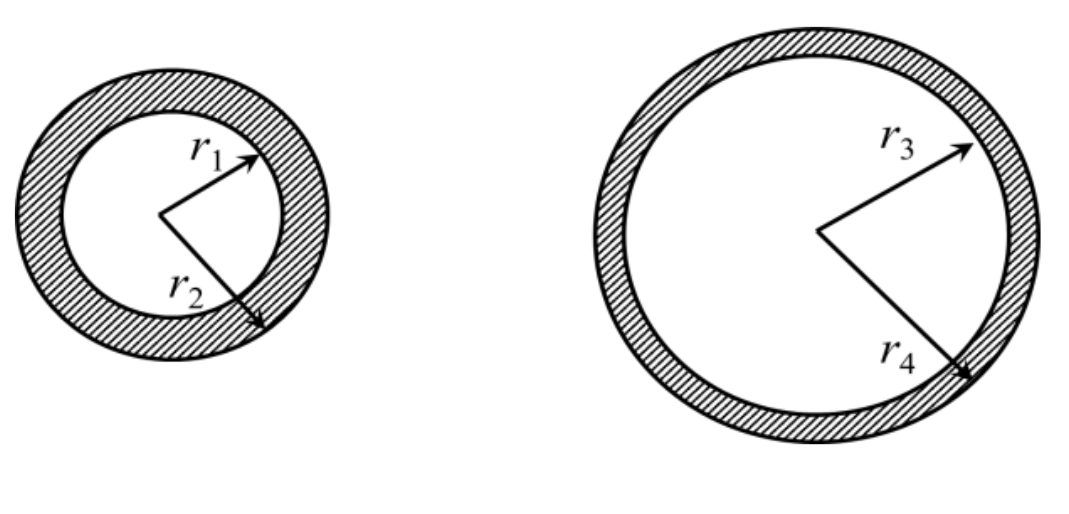
\includegraphics[scale=0.3]{q8}
              \caption{Figure for Q.8}
              \label{q8}
          \end{figure}

          \begin{enumerate}

              \begin{multicols}{4}

                  \item $> 1$\columnbreak

                  \item $< 0.5$\columnbreak

                  \item $=1$\columnbreak

                  \item \text{between 0.5 and 1}

              \end{multicols}

          \end{enumerate}

    \item A cantilever beam having square cross-section of side $a$ is subjected to an end load. If $a$ is increased by 19\%, the tip deflection decreases approximately by

          \begin{enumerate}

              \begin{multicols}{4}

                  \item 19\%

                  \item 29\%

                  \item 41\%

                  \item 50\%

              \end{multicols}

          \end{enumerate}

    \item A car is moving on a curved horizontal road of radius 100 m with a speed of 20 m/s. The rotating masses of the engine have an angular speed of 100 rad/s in clockwise direction when viewed from the front of the car. The combined moment of inertia of the rotating masses is 10 kg-m$^2$. The magnitude of the gyroscopic moment (in N-m) is \_\_\_\_\_\_\_\_

    \item A single degree of freedom spring mass system with viscous damping has a spring constant of 10 kN/m. The system is excited by a sinusoidal force of amplitude 100 N. If the damping factor (ratio) is 0.25, the amplitude of steady state oscillation at resonance is \_\_\_\_\_\_\_\_ mm.

    \item The spring constant of a helical compression spring DOES NOT depend on

          \begin{enumerate}

              \item coil diameter

              \item material strength

              \item number of active turns

              \item wire diameter

          \end{enumerate}

    \item The instantaneous stream-wise velocity of a turbulent flow is given as follows:
          \begin{align}
              u(x,y,z,t) = \bar{u}(x,y,z) + u'(x,y,z,t)
          \end{align}

          The time-average of the fluctuating velocity $u'(x,y,z,t)$ is

          \begin{enumerate}

              \begin{multicols}{4}

                  \item $u'/2$

                  \item $-\bar{u}/2$

                  \item zero

                  \item $\bar{u}/2$

              \end{multicols}

          \end{enumerate}

    \item For a floating body, buoyant force acts at the

          \begin{enumerate}

              \item centroid of the floating body

              \item center of gravity of the body

              \item centroid of the fluid vertically below the body

              \item centroid of the displaced fluid

          \end{enumerate}

    \item A plastic sleeve of outer radius $r_0 = 1$ mm covers a wire (radius $r = 0.5$ mm) carrying electric current. Thermal conductivity of the plastic is 0.15 W/m-K. The heat transfer coefficient on the outer surface of the sleeve exposed to air is 25 W/m$^2$-K. Due to the addition of the plastic cover, the heat transfer from the wire to the ambient will

          \begin{enumerate}

              \item increase

              \item remain the same

              \item decrease

              \item be zero

          \end{enumerate}

    \item Which of the following statements are TRUE with respect to heat and work?

          (i) They are boundary phenomena

          (ii) They are exact differentials

          (iii) They are path functions

          \begin{enumerate}

              \item both (i) and (ii)

              \item both (i) and (iii)

              \item both (ii) and (iii)

              \item only (iii)

          \end{enumerate}

    \item Propane (C$_3$H$_8$) is burned in an oxygen atmosphere with 10\% deficit oxygen with respect to the stoichiometric requirement. Assuming no hydrocarbons in the products, the volume percentage of CO in the products is \_\_\_\_\_\_\_\_

    \item Consider two hydraulic turbines having identical specific speed and effective head at the inlet. If the speed ratio ($N_1/N_2$) of the two turbines is 2, then the respective power ratio ($P_1/P_2$) is \_\_\_\_\_\_\_\_

    \item The INCORRECT statement about regeneration in vapor power cycle is that

          \begin{enumerate}

              \item it increases the irreversibility by adding the liquid with higher energy content to the steam generator

              \item heat is exchanged between the expanding fluid in the turbine and the compressed fluid before heat addition

              \item the principle is similar to the principle of Stirling gas cycle

              \item it is practically implemented by providing feed water heaters

          \end{enumerate}

    \item The "Jominy test" is used to find

          \begin{enumerate}

              \begin{multicols}{2}

                  \item Young's modulus

                  \item hardenability\columnbreak

                  \item yield strength

                  \item thermal conductivity

              \end{multicols}

          \end{enumerate}

    \item Under optimal conditions of the process the temperatures experienced by a copper work piece in fusion welding, brazing and soldering are such that

          \begin{enumerate}

              \item $T_{\text{welding}} > T_{\text{soldering}} > T_{\text{brazing}}$

              \item $T_{\text{soldering}} > T_{\text{welding}} > T_{\text{brazing}}$

              \item $T_{\text{brazing}} > T_{\text{welding}} > T_{\text{soldering}}$

              \item $T_{\text{welding}} > T_{\text{brazing}} > T_{\text{soldering}}$

          \end{enumerate}

    \item The part of a gating system which regulates the rate of pouring of molten metal is

          \begin{enumerate}

              \begin{multicols}{4}

                  \item pouring basin

                  \item runner

                  \item choke

                  \item ingate

              \end{multicols}

          \end{enumerate}

    \item The non-traditional machining process that essentially requires vacuum is

          \begin{enumerate}

              \item electron beam machining

              \item electro chemical machining

              \item electro chemical discharge machining

              \item electro discharge machining

          \end{enumerate}

    \item In an orthogonal cutting process the tool used has rake angle of zero degree. The measured cutting force and thrust force are 500 N and 250 N, respectively. The coefficient of friction between the tool and the chip is \_\_\_\_\_\_\_\_

    \item Match the following:

          \begin{table}[H]
              \centering
              \begin{tabular}{|l|l|l|l|}
                  \hline
                  P. & Feeler gauge           & I.   & Radius of an object                  \\
                  Q. & Fillet gauge           & II.  & Diameter within limits by comparison \\
                  R. & Snap gauge             & III. & Clearance or gap between components  \\
                  S. & Cylindrical plug gauge & IV.  & Inside diameter of straight hole     \\
                  \hline
              \end{tabular}
              \label{t25}
          \end{table}

          \begin{enumerate}

              \item P–III, Q–I, R–II, S–IV

              \item P–III, Q–II, R–I, S–IV

              \item P–IV, Q–II, R–I, S–III

              \item P–IV, Q–I, R–II, S–III

          \end{enumerate}

\end{enumerate}

\normalsize\textbf{Q. 26 – Q. 55 carry two marks each.}\\

\begin{enumerate}[resume]

    \item Consider the function $f(x) = x^3 - 6x^2 + 9x + 25$ in the domain $[1, 10]$. The global minimum of $f(x)$ is \_\_\_\_\_\_\_\_

    \item If $y(x)$ satisfies the boundary value problem $y'' + \lambda^2 y = 0$, $y(0) = 0$, $y(\pi) = \sqrt{2}$, then $y(\pi/4)$ is \_\_\_\_\_\_\_\_

    \item The value of the integral
          \begin{align}
              \int_{-\infty}^{\infty} \frac{\sin x}{x^2 + 2x + 2} dz
          \end{align}
          evaluated using contour integration and the residue theorem is

          \begin{enumerate}

              \begin{multicols}{4}

                  \item $-\pi \sin(1)/e$

                  \item $-\pi \cos(1)/e$

                  \item $\sin(1)/e$

                  \item $\cos(1)/e$

              \end{multicols}

          \end{enumerate}

    \item Gauss-Seidel method is used to solve the following equations (as per the given order):
          \begin{align}
              x_1 + 4x_2 + 8x_3 & = 12 \\
              2x_1 + x_2 + x_3  & = 5  \\
              x_1 + x_2 + x_3   & = 6
          \end{align}

          Assuming initial guess as $x_1 = x_2 = x_3 = 0$, the value of $x_2$ after the first iteration is \_\_\_\_\_\_\_\_

    \item A block of mass $m$ rests on an inclined plane and is attached by a string to the wall as shown in the figure. The coefficient of static friction between the plane and the block is 0.25. The string can withstand a maximum force of 20 N. The maximum value of the mass (m) for which the string will not break and the block will be in static equilibrium is \_\_\_\_\_\_\_\_ kg.

          Take $\cos \theta = 0.8$ and $\sin \theta = 0.6$

          Acceleration due to gravity $g = 10$ m/s$^2$

          \begin{figure}[H]
              \centering
              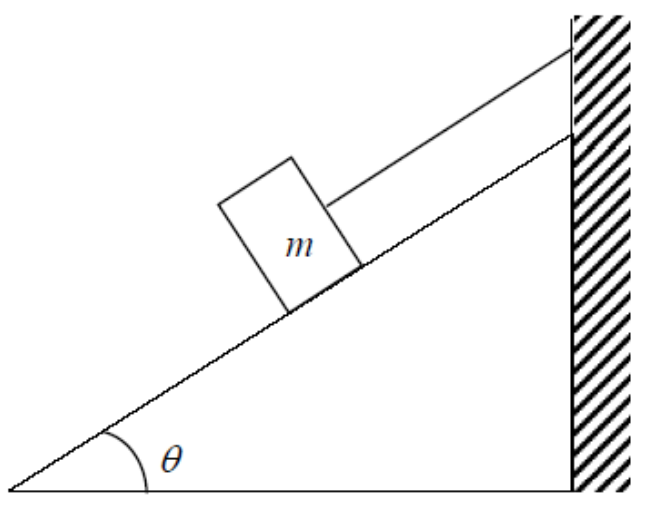
\includegraphics[scale=0.3]{q30}
              \caption{Figure for Q.30}
              \label{q30}
          \end{figure}

    \item A two-member truss PQR is supporting a load W. The axial forces in members PQ and QR are respectively

          \begin{figure}[H]
              \centering
              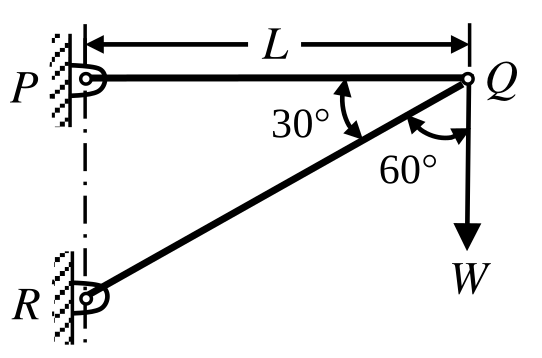
\includegraphics[scale=0.3]{q31}
              \caption{Figure for Q.31}
              \label{q31}
          \end{figure}

          \begin{enumerate}

              \item $2W$ tensile and $\sqrt{3}W$ compressive

              \item $\sqrt{3}W$ tensile and $2W$ compressive

              \item $\sqrt{3}W$ compressive and $2W$ tensile

              \item $2W$ compressive and $\sqrt{3}W$ tensile

          \end{enumerate}

    \item A horizontal bar with a constant cross-section is subjected to loading as shown in the figure. The Young's moduli for the sections AB and BC are 3E and E, respectively.

          \begin{figure}[H]
              \centering
              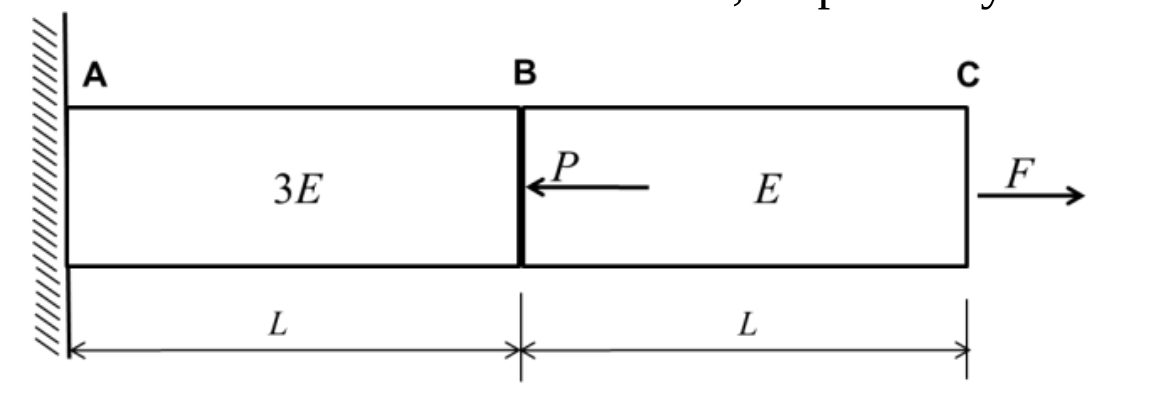
\includegraphics[scale=0.3]{q32}
              \caption{Figure for Q.32}
              \label{q32}
          \end{figure}

          For the deflection at C to be zero, the ratio P/F is \_\_\_\_\_\_\_\_

    \item The figure shows cross-section of a beam subjected to bending. The area moment of inertia (in mm$^4$) of this cross-section about its base is \_\_\_\_\_\_\_\_

          \begin{figure}[H]
              \centering
              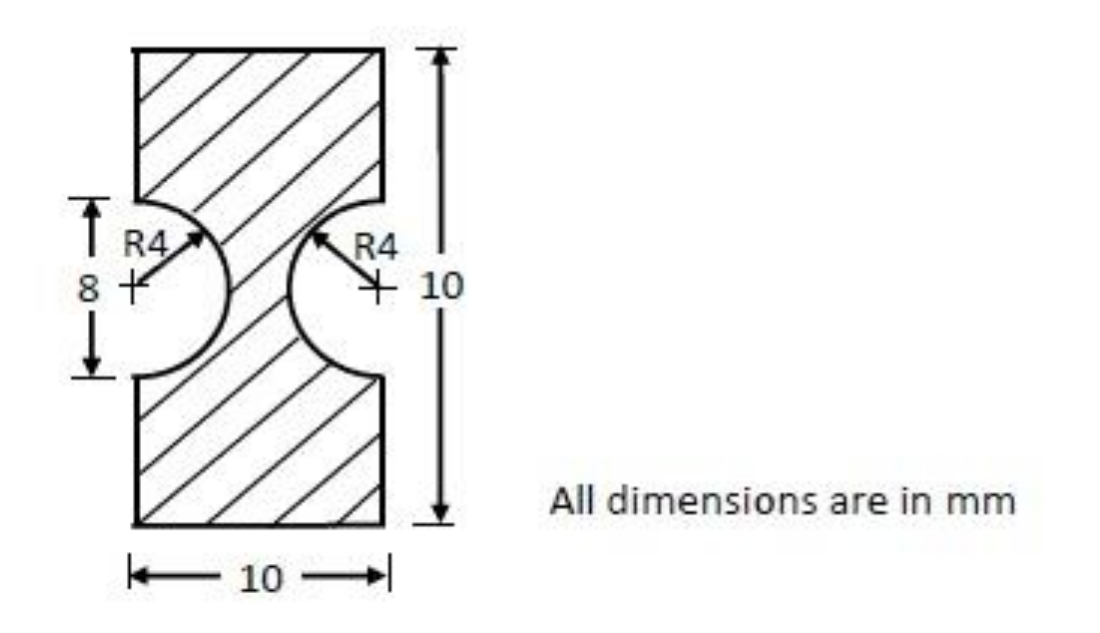
\includegraphics[scale=0.2]{q33}
              \caption{Figure for Q.33}
              \label{q33}
          \end{figure}

    \item A simply-supported beam of length 3L is subjected to the loading shown in the figure.

          \begin{figure}[H]
              \centering
              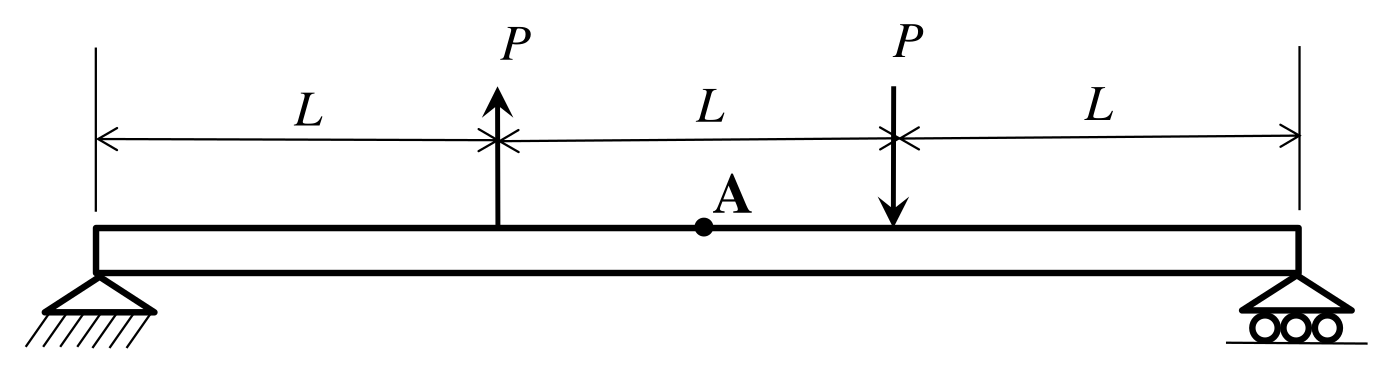
\includegraphics[scale=0.3]{q34}
              \caption{Figure for Q.34}
              \label{q34}
          \end{figure}

          It is given that P = 1 N, L = 1 m and Young's modulus E = 200 GPa. The cross-section is a square with dimension 10 mm × 10 mm. The bending stress (in Pa) at the point A located at the top surface of the beam at a distance of 1.5L from the left end is \_\_\_\_\_\_\_\_

          (Indicate compressive stress by a negative sign and tensile stress by a positive sign.)

    \item A slider crank mechanism with crank radius 200 mm and connecting rod length 800 mm is shown. The crank is rotating at 600 rpm in the counterclockwise direction. In the configuration shown, the crank makes an angle of 90° with the sliding direction of the slider, and a force of 5 kN is acting on the slider. Neglecting the inertia forces, the turning moment on the crank (in kN-m) is \_\_\_\_\_\_\_\_

          \begin{figure}[H]
              \centering
              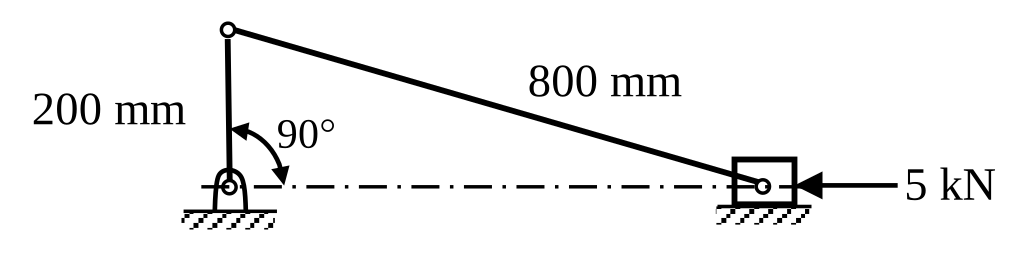
\includegraphics[scale=0.3]{q35}
              \caption{Figure for Q.35}
              \label{q35}
          \end{figure}

    \item In the gear train shown, gear 3 is carried on arm 5. Gear 3 meshes with gear 2 and gear 4. The number of teeth on gear 2, 3, and 4 are 60, 20, and 100, respectively. If gear 2 is fixed and gear 4 rotates with an angular velocity of 100 rpm in the counterclockwise direction, the angular speed of arm 5 (in rpm) is

          \begin{figure}[H]
              \centering
              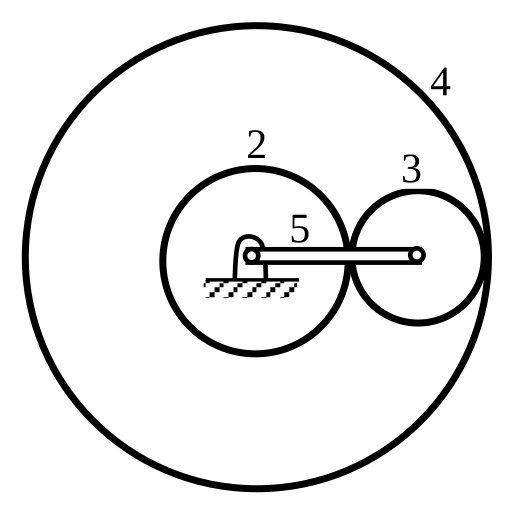
\includegraphics[scale=0.3]{q36}
              \caption{Figure for Q.36}
              \label{q36}
          \end{figure}

          \begin{enumerate}

              \item 166.7 counterclockwise

              \item 166.7 clockwise

              \item 62.5 counterclockwise

              \item 62.5 clockwise

          \end{enumerate}

    \item A solid disc with radius $a$ is connected to a spring at a point $d$ above the center of the disc. The other end of the spring is fixed to the vertical wall. The disc is free to roll without slipping on the ground. The mass of the disc is M and the spring constant is K. The polar moment of inertia for the disc about its centre is $J = \frac{Ma^2}{2}$.

          \begin{figure}[H]
              \centering
              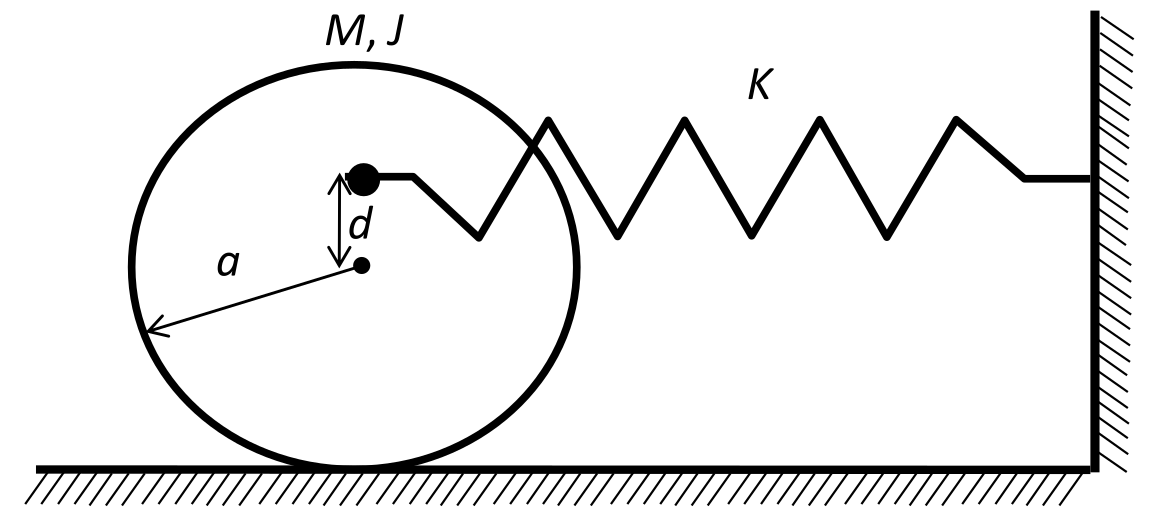
\includegraphics[scale=0.3]{q37}
              \caption{Figure for Q.37}
              \label{q37}
          \end{figure}

          The natural frequency of this system in rad/s is given by

          \begin{enumerate}

              \item $\sqrt{\frac{2K(a + d)}{3Ma^2}}$

              \item $\sqrt{\frac{2K}{3M}}$

              \item $\sqrt{\frac{2K(a + d)}{Ma^2}}$

              \item $\sqrt{\frac{K(a + d)}{Ma^2}}$

          \end{enumerate}

    \item The principal stresses at a point inside a solid object are $\sigma_1 = 100$ MPa, $\sigma_2 = 100$ MPa and $\sigma_3 = 0$ MPa. The yield strength of the material is 200 MPa. The factor of safety calculated using Tresca (maximum shear stress) theory is $n_T$ and the factor of safety calculated using von Mises (maximum distortional energy) theory is $n_V$. Which one of the following relations is TRUE?

          \begin{enumerate}

              \item $n_T = (\sqrt{3}/2)n_V$

              \item $n_T = (\sqrt{2})n_V$

              \item $n_T = n_V$

              \item $n_V = (\sqrt{3})n_T$

          \end{enumerate}

    \item An inverted U-tube manometer is used to measure the pressure difference between two pipes A and B, as shown in the figure. Pipe A is carrying oil (specific gravity = 0.8) and pipe B is carrying water. The densities of air and water are 1.16 kg/m$^3$ and 1000 kg/m$^3$, respectively. The pressure difference between pipes A and B is \_\_\_\_\_\_\_\_ kPa.\\
          \textbf{Acceleration due to gravity g = 10 m/s$^2$.}
          \begin{figure}[H]
              \centering
              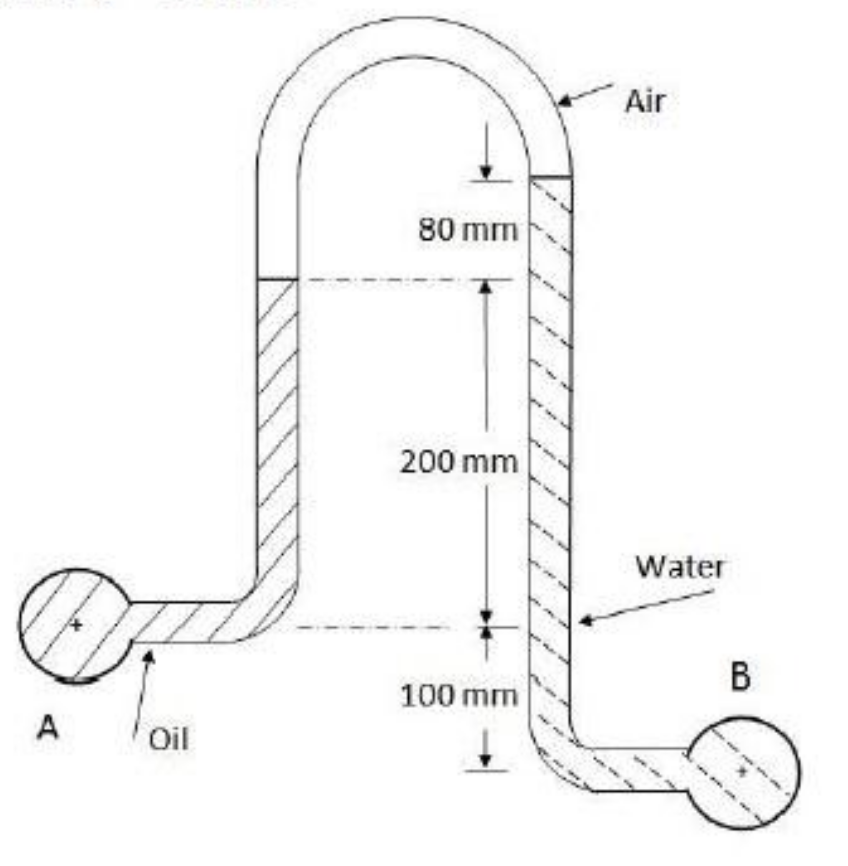
\includegraphics[scale=0.3]{q39}
              \caption{}
              \label{q39}
          \end{figure}

    \item Oil (kinematic viscosity, $\nu = 10^{-4}$ m$^2$/s) flows through a pipe of 0.5 m diameter with a velocity of 10 m/s. Water (kinematic viscosity, $\nu = 10^{-6}$ m$^2$/s) is flowing through a model pipe of diameter 20 mm. For satisfying the dynamic similarity, the velocity of water (in m/s) is \_\_\_\_\_\_\_\_

    \item A steady laminar boundary layer is formed over a flat plate as shown in the figure. The free stream velocity of the fluid is $U_0$. The velocity profile at the inlet a-b is uniform, while that at a downstream location c-d is given by $u = U_o \left[ 2(\frac{y}{\delta}) - (\frac{y}{\delta})^2 \right] $.

          \begin{figure}[H]
              \centering
              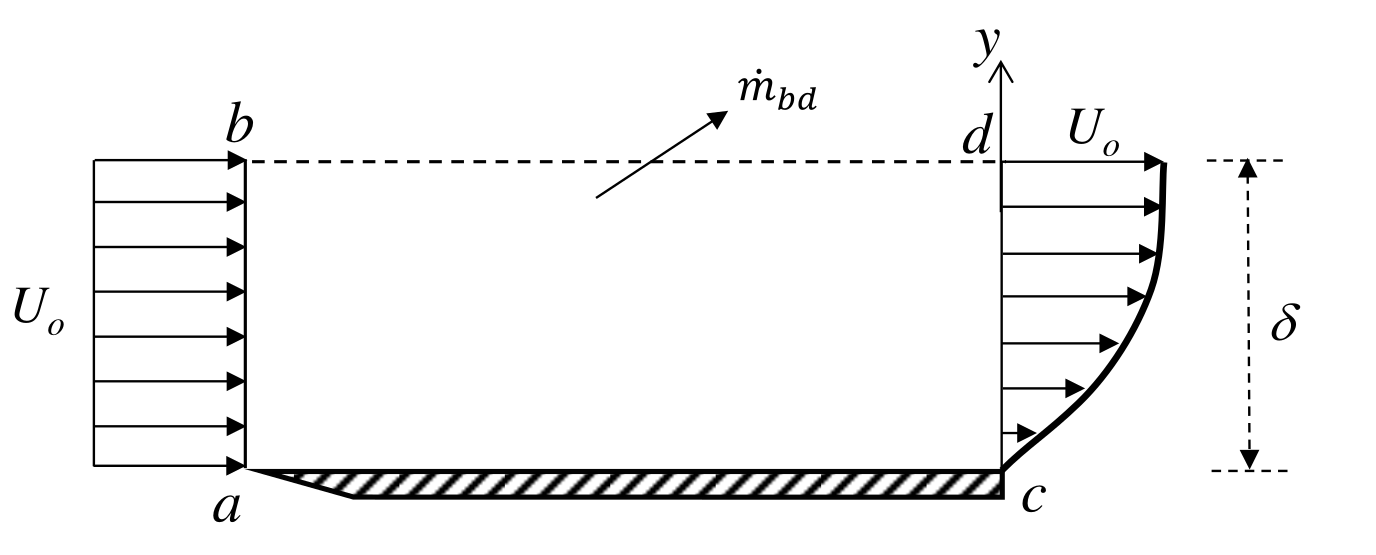
\includegraphics[scale=0.25]{q41}
              \caption{Figure for Q.41}
              \label{q41}
          \end{figure}

          The ratio of the mass flow rate, $\dot{m}_{bd}$, leaving through the horizontal section b-d to that entering through the vertical section a-b is \_\_\_\_\_\_\_\_

    \item A steel ball of 10 mm diameter at 1000 K is required to be cooled to 350 K by immersing it in a water environment at 300 K. The convective heat transfer coefficient is 1000 W/m$^2$-K. Thermal conductivity of steel is 40 W/m-K. The time constant for the cooling process is 16 s. The time required (in s) to reach the final temperature is \_\_\_\_\_\_\_\_

    \item An infinitely long furnace of 0.5 m × 0.4 m cross-section is shown in the figure below. Consider all surfaces of the furnace to be black. The top and bottom walls are maintained at temperature $T_1 = T_3 = 927°C$ while the side walls are at temperature $T_2 = T_4 = 527°C$. The view factor, $F_{1-2}$ is 0.26. The net radiation heat loss or gain on side 1 is \_\_\_\_\_\_\_\_ W/m.

          Stefan-Boltzmann constant = $5.67 \times 10^{-8}$ W/m$^2$-K$^4$

          \begin{figure}[H]
              \centering
              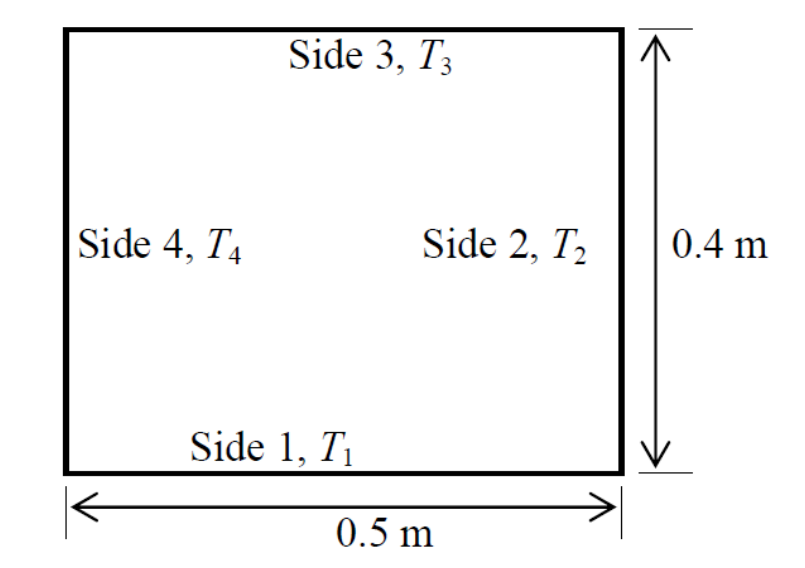
\includegraphics[scale=0.3]{q43}
              \caption{Figure for Q.43}
              \label{q43}
          \end{figure}

    \item A fluid (Prandtl number, Pr = 1) at 500 K flows over a flat plate of 1.5 m length, maintained at 300 K. The velocity of the fluid is 10 m/s. Assuming kinematic viscosity, $\nu = 5 \times 10^{-5}$ m$^2$/s, the thermal boundary layer thickness (in mm) at 0.5 m from the leading edge is \_\_\_\_\_\_\_\_

    \item For water at 25°C, $dp_{s}/dT_{s} = 0.189$ kPa/K ($p_{s}$ is the saturation pressure in kPa and $T_{s}$ is the saturation temperature in K) and the specific volume of dry saturated vapour is 43.38 m$^3$/kg. Assume that the specific volume of liquid is negligible in comparison with that of vapour. Using the Clausius-Clapeyron equation, an estimate of the enthalpy of evaporation of water at 25°C (in kJ/kg) is \_\_\_\_\_\_\_\_

    \item An ideal gas undergoes a reversible process in which the pressure varies linearly with volume. The conditions at the start (subscript 1) and at the end (subscript 2) of the process with usual notation are: $p_1 = 100$ kPa, $V_1 = 0.2$ m$^3$ and $p_2 = 200$ kPa, $V_2 = 0.1$ m$^3$ and the gas constant, $R = 0.275$ kJ/kg-K. The magnitude of the work required for the process (in kJ) is \_\_\_\_\_\_\_\_

    \item In a steam power plant operating on an ideal Rankine cycle, superheated steam enters the turbine at 3 MPa and 350°C. The condenser pressure is 75 kPa. The thermal efficiency of the cycle is \_\_\_\_\_\_\_\_ percent.

          Given data:
          For saturated liquid, at P = 75 kPa,
          $h_f = 384.39$ kJ/kg, $v_f = 0.001037$ m$^3$/kg, $s_f = 1.213$ kJ/kg-K
          At 75 kPa, $h_{fg} = 2278.6$ kJ/kg, $s_{fg} = 6.2434$ kJ/kg-K
          At P = 3 MPa and T = 350°C (superheated steam),
          $h = 3115.3$ kJ/kg, $s = 6.7428$ kJ/kg-K

    \item A hypothetical engineering stress-strain curve shown in the figure has three straight lines PQ, QR, RS with coordinates P(0,0), Q(0.2,100), R(0.6,140) and S(0.8,130). 'Q' is the yield point, 'R' is the UTS point and 'S' the fracture point.

          \begin{figure}[H]
              \centering
              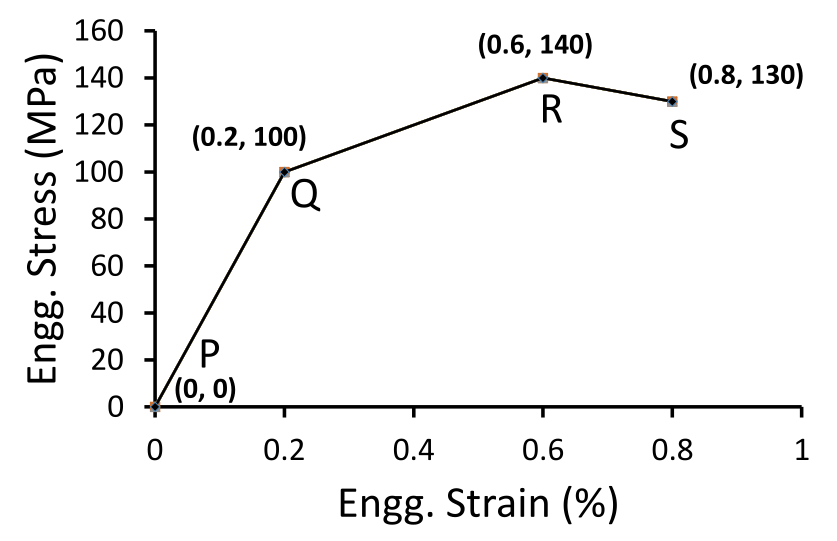
\includegraphics[scale=0.3]{q48}
              \caption{Figure for Q.48}
              \label{q48}
          \end{figure}

          The toughness of the material (in MJ/m$^3$) is \_\_\_\_\_\_\_\_

    \item Heat is removed from a molten metal of mass 2 kg at a constant rate of 10 kW till it is completely solidified. The cooling curve is shown in the figure.
          \begin{figure}[H]
              \centering
              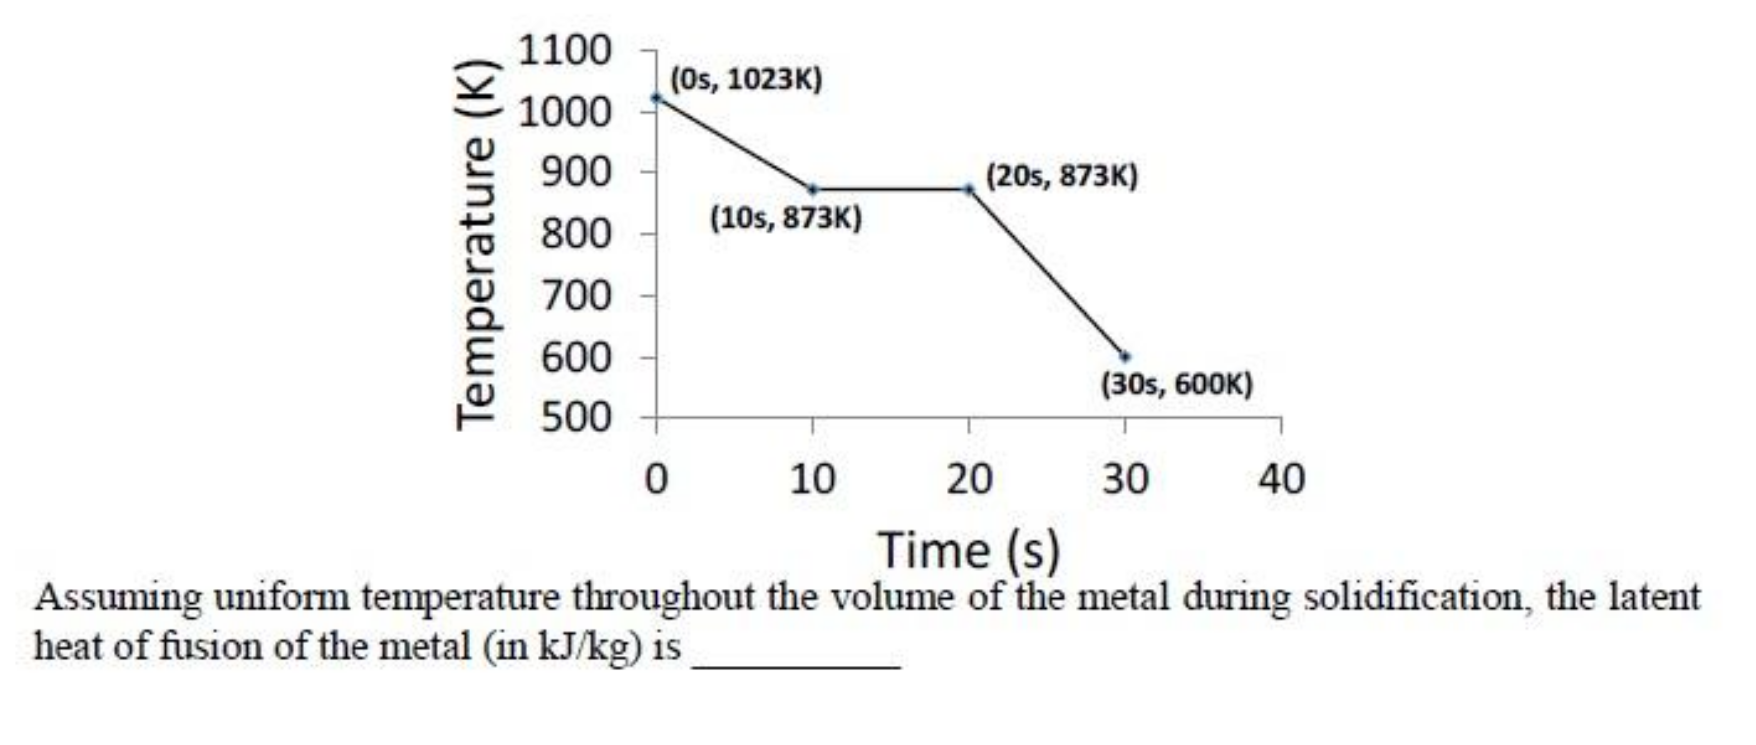
\includegraphics[scale=0.23]{q49}
              \caption{Figure for Q.49}
              \label{q49}
          \end{figure}

    \item The tool life equation for HSS tool is $VT^{0.125}f^{0.77}d^{0.37} = C$. The tool life (T) of 30 min is obtained using the following cutting conditions:
          V = 45 m/min, f = 0.35 mm, d = 2.0 mm
          If speed (V), feed (f) and depth of cut (d) are increased individually by 25\%, the tool life (in min) is

          \begin{enumerate}

              \begin{multicols}{4}

                  \item 0.15

                  \item 1.06

                  \item 22.50

                  \item 30.0

              \end{multicols}

          \end{enumerate}

    \item A cylindrical job with diameter of 200 mm and height of 100 mm is to be cast using modulus method of riser design. Assume that the bottom surface of cylindrical riser does not contribute as cooling surface. If the diameter of the riser is equal to its height, then the height of the riser (in mm) is

          \begin{enumerate}

              \begin{multicols}{4}

                  \item 150

                  \item 200

                  \item 100

                  \item 125

              \end{multicols}

          \end{enumerate}

    \item A 300 mm thick slab is being cold rolled using roll of 600 mm diameter. If the coefficient of friction is 0.08, the maximum possible reduction (in mm) is \_\_\_\_\_\_\_\_

    \item The figure below represents a triangle PQR with initial coordinates of the vertices as P(1,3), Q(4,5) and R(5,3.5). The triangle is rotated in the X-Y plane about the vertex P by angle $\theta$ in clockwise direction. If $\sin \theta = 0.6$ and $\cos \theta = 0.8$, the new coordinates of the vertex Q are

          \begin{enumerate}

              \begin{multicols}{4}

                  \item (4.6, 2.8)

                  \item (3.2, 4.6)

                  \item (7.9, 5.5)

                  \item (5.5, 7.9)

              \end{multicols}

          \end{enumerate}

    \item The annual demand for an item is 10,000 units. The unit cost is Rs. 100 and inventory carrying charges are 14.4\% of the unit cost per annum. The cost of one procurement is Rs. 2000. The time between two consecutive orders to meet the above demand is \_\_\_\_\_\_\_\_ month(s).

    \item Maximize $Z=15X_1 + 20X_2$
          subject to
          \begin{align}
              12X_1 + 4X_2 & \geq 36 \\
              12X_1 - 6X_2 & \leq 24 \\
              X_1, X_2     & \geq 0
          \end{align}

          The above linear programming problem has

          \begin{enumerate}

              \item infeasible solution

              \item unbounded solution

              \item alternative optimum solutions

              \item degenerate solution

          \end{enumerate}

\end{enumerate}

\vspace{1cm}

\centering\Large\textbf{END OF THE QUESTION PAPER}

\end{document}